\chapter{Zone d'édition}

	\section{Contrôles}

		\subsection{Déplacement}

			L'application fournis une zone d'édition relativement large. Il est possible de naviguer dans celle-ci de deux manière. Soit en utilisant les barres de navigation sur les bord la zone, soit en maintenant le clique gauche tout en déplaçant la souris.

		\subsection{Niveau de zoom}

			Il est possible d'obtenir une vue beaucoup plus générale du livre et des différents noeuds. Pour cela il suffit d'utiliser la molette de la souris.

	\section{Le prélude}

        Le prélude permet comme son nom l'indique de gérer le texte de départ du livre. Il est symbolisé par le carré fushia en haut à gauche. Cependant, celui-ci permet également de gérer deux éléments supplémentaires : La conception de la "phase de création du personnage" ainsi que l'édition du personnage principal.

		Commençons d'abord par accéder à la boite de dialogue qui permet d'ajuster les différents éléments cités précédemment. Tout d'abord, il faut sélectionner le mode 
\includegraphics[height=10pt]{img/icons/select.png}, puis double cliquer sur le prélude.

		La boite de dialogue suivante devient alors visible.

		\begin{figure}[H]
			\centering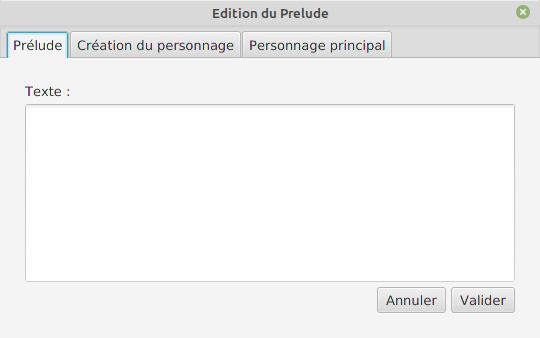
\includegraphics[width=0.4\textwidth, keepaspectratio]{img/prelude.png}
		\end{figure}

		Trois onglets sont disponibles. Le premier, "Prélude", permet de définir le texte à afficher au tout début du livre. Il permet de situer le lecteur dans l'univers de ce qu'il va lire. Le deuxième, "Création du peronnage" permet au lecteur de faire différents choix concernant son personnage, que cela soit sur les compétences qu'il possèdera, les items avec lesquels il débutera ou encore les items supplémentaires qu'il peut acheter. Et enfin, "Personnage Principal" qui permet de définir les caractéristiques de celui-ci.

		Nous ne détaillerons pas l'onglet concernant le Prélude car celui-ci est suffisement explicite.

		\subsection{Création du personnage}
			Cette onglet à un bouton 
\includegraphics[height=10pt, keepaspectratio]{img/ajouterBouton.png}, permettant d'ajouter une étape, dans la conception du personnage, étape visible sur l'image ci-dessous.

			\begin{figure}[H]
				\centering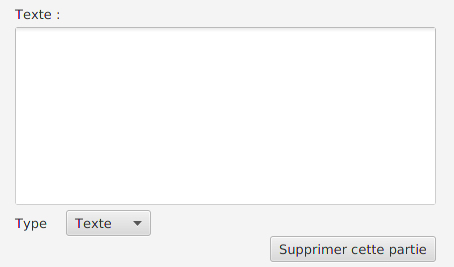
\includegraphics[width=0.4\textwidth, keepaspectratio]{img/etapeConceptionPerso.png}
			\end{figure}

			La zone de tete permet d'introduire le choix que le joueur doit effectuer tandis que la liste déroulante permet de sélectionner le type de cette étape. Il est important d'avoir déjà ajouter des items ou compétences pour voir cette liste (cf : \nameref{chapter:elementsConstitutifLivre} page \pageref{chapter:elementsConstitutifLivre}).

			Le bouton 
\includegraphics[height=10pt, keepaspectratio]{img/preludeSupprimerBouton.png} permet de supprimer l'étape.

			\subsubsection{Le type item / shop}
				\phantomsection\label{subsubsec:item_shop}

				Une liste déroulante s'affiche avec tout les items encore non sélectionné. Pour ajouter un item, il faut d'abord en sélectionner un, puis cliquer sur le bouton 
\includegraphics[height=10pt, keepaspectratio]{img/ajouterBouton.png}. Une fois l'item ajouté, il peut-être supprimé en faisant apparaitre le menu grâce à un clique droit sur celui-ci.

				L'utilisateur peut aussi le sélectionner afin de renseigner changer certaines informations :

				\begin{description}
					\item[Type Item :] Le nombre d'item disponible
					\item[Type Shop :] Le nombre d'item disponible à la vente, ainsi que son prix d'achat et son prix de revente
				\end{itemize}

				Si un champ est changé, l'utilisateur doit alors cliquer sur le bouton modifier pour prendre en compte les changements, ce sans quoi, ils seront simplement ignorés.

			\subsubsection{Le type compétence}
				\phantomsection \label{subsubsec:persoCreationSkill}

				Le bouton 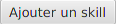
\includegraphics[height=10pt, keepaspectratio]{img/preludeAjouterSkillBouton.png} affiche une liste déroulante permettant de sélectionner la compétence que l'on souhaite rendre disponible dans le choix du joueur. Si l'on souhaite supprimer l'une des compétences il suffit de sélectionner l'élément vide et de valider les modifications sur la boite de dialogue.

		\subsection{Personnage principal}
			\label{subsec:main_character}

			L'affichage est casiment identique à celui concernant l'ajout d'un personnage basique (cf : \nameref{sec:perso} page \pageref{sec:perso}). Quelques champs supplémentaires sontt présent comme la quantité d'items pouvant être porté et la somme qu'il possède au départ.

	\section{Les noeuds}

		\label{chapter:noeuds}
		La création d'un noeud se fait à partir du mode 
\includegraphics[height=10pt]{img/modeEdition.png}. Ce mode permet de créer un paragraphe. Une fois le mode sélectionné, il faut alors cliquer n'importe où dans la zone d'édition. Une fenêtre va alors apparaître.

		\subsection{Noeuds à choix}
			Ces noeuds contiennent trois onglets: édition du noeud (\textit{Noeud}), ajout des items à prendre (\textit{Item}), ajout des items à acheter (\textit{Shop}).

			\begin{itemize}
				\item \textbf{Noeud} : contient un paragraphe, un champ de texte de gain/perte de vie, un champ de texte permettant à l'utilisateur de définir un nombre maximum d'item à prendre/acheter sur ce noeud.
				\begin{center}
					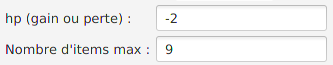
\includegraphics[height=1cm]{img/noeudBasic.png}
				\end{center}

				\item \textbf{Item} et \textbf{Shop} : voir la subsection  \nameref{subsubsec:item_shop} à la page \pageref{subsubsec:item_shop}. Des items doivent être créé pour être sélectionné (Voir le chapitre \ref{chapter:inclus} à la page \pageref{chapter:inclus}).
			\end{itemize}

			Tout les champs des noeuds, sauf le champ contenant le paragraphe (\textit{Texte}), ne peut contenir des lettres.

			\subsubsection{Noeud basic}
				Ce noeud permet d'avoir un simple paragraphe à choix.

			\subsubsection{Noeud aléatoire}
				Ce noeud ne diffère pas du noeud basique sur sa présentation, mais à la création de son/ses lien(s) (voir la section \ref{subsection:lienAléatoire} à la page \pageref{subsection:lienAléatoire}).

			\subsubsection{Noeud combat}\phantomsection\label{subsubsec:combat}
				Ce noeud contient deux nouvelle données à remplir. Tout d'abord, l'utilisateu peut définir le nombre de tours avant évasion. Puis il y a un bouton 
\includegraphics[height=10pt]{img/noeudAddPersonnage} permettant d'ajouter des ennemis grâce à une liste déroulante qui apparait. Chaque ennemis peut être ajouter plusieurs fois permettant ainsi de laisser la liberté à l'utilisateur d'avoir plusieurs même ennemis. Pour choisir un ennemis, il doit d'abord être créé (Voir le chapitre \ref{chapter:inclus} à la page \pageref{chapter:inclus})
				Ce noeud diffère également lors de la création de son/ses lien(s) (voir la section \ref{subsection:lienCombat} à la page \pageref{subsection:lienCombat}).

		\subsection{Noeud terminaux}
			Ces noeuds permettent de définir si le joueur a gagné ou perdu. Le livre est donc fini à cette endroit. Le livre ne peut pas être lancé tant que tout les noeuds ne finissent pas sur un noeud terminal. En effet, il est impossible au joueur de terminer sur un autre noeud qu'un noeud terminal.

		\subsection{Modification des noeuds}
			Ces différents noeuds présentés sont modifiables à l'aide du mode 
\includegraphics[height=0.4cm]{img/modeSelected.png}. Un double clique est nécessaire afin de pouvoir éditer le noeud voulu.

		\subsection{Positionnement des noeuds}
			Les noeuds peuvent être déplacés grâce au mode 
\includegraphics[height=10pt]{img/modeSelected.png}. Un simple clique/glisse suffit pour déplacer n'importe quel noeud.

		\subsection{Supression des noeuds}
			Ces noeuds, sauf le prélude, peuveut être supprimés à l'aide du mode 
\includegraphics[height=0.4cm]{img/modeSupression.png}. Un simple clique sur le noeud est alors necessaire. Une boite de dialog va alors s'ouvrir permettant de vérifier si l'utilisateur est bien sûr de son action. Attention, si des liens étaient présent sur ce noeud, ils sont tout simplement supprimés.

	\section{Lien entre les noeuds}\label{chapter:lien}
	\label{sec:prerequis}

	\subsection{Lien prélude-noeud}
		Ce lien est très important. Il permet à l'utilisateur d'utiliser toutes les options possible dans la barre de menu, dans l'onglet "\textit{Livre}". Cela permet d'indiquer le premier noeud qui va être lu, après le prélude. Ce noeud peut être tracé grâce au mode 
\includegraphics[height=10pt]{img/modePreludeNoeud.png} même si le prélude n'est pas complété. En effet, le joueur va alors avoir un personnage préétabli.
		Une fois le mode selectionné, un simple clique sur un carré est nécessaire. Si l'utilisateur veut changer le premier noeud, le même mode 
\includegraphics[height=10pt]{img/modePreludeNoeud.png} doit être sélectionné, et le même procédé est nécessaire.

	\subsection{Lien entre les noeuds}
		Ces liens permettent de relier un paragraphe à un autre paragraphe grâce à un choix. Ce lien ne peut pas commencer sur un noeud terminal, ni sur le prélude. Tant que tout les liens ne sont pas créés, il est impossible de jouer, ni d'estimer la difficulté.\\

		Pour tracer ce lien, le mode 
\includegraphics[height=10pt]{img/modeLien.png} est requis. L'utilisateur doit alors cliquer sur un premier noeud, puis sur un deuxième. Ce noeud peut être le même afin de laisser la liberté de créer une boucle si necessaire.
		Si le permier clique n'était pas voulu, un simple clique dans la zone vide d'édition est requis pour annulé le premier clique.\\

		Une fois ce lien trâcé, une boite de dialog apparait. Elle contient un texte qui s'affichera lors de l'affichage de tout les choix, deux champs de texte de gain/perte de point de vie et de monnaie, ainsi que d'un onglet contenant les prérequis. Une coche est également disponible permettant de prendre toujours ce choix automatiquemenent.
		Ces prérequis permettent à l'utilisateur de créer des choix où il est possible d'y accèder que si certains objets/compétences sont possédés par le joueur.
		Pour cela, un bouton 
\includegraphics[height=10pt]{img/ajouterBouton.png} permet de créer des listes de prérequis. Comme par exemple, le joueur doit posséder l'épée "Excalibur" ainsi que le bouclier "Pavois" \textbf{ou} trois d'argent ainsi que la compétence "Boule de feu" et l'épée "Excalibur".
		Pour l'ajout de ces items/monnaie/compétences, c'est le même procédé que \ref{subsubsec:compétences} et \ref{subsubsec:item_shop}.\\

		Tout les champs des liens, sauf le champ contenant le texte du choix (\textit{Texte}), ne peut contenir des lettres et ne peut être vide. L'utilisateur ne peut valider que si ces conditions sont remplis. S'il décide d'annuler, toutes les modifications seront perdu.\\

	\subsection{Lien noeud combat}\label{subsection:lienCombat}
		\begin{minipage}{0.70\textwidth}
			Si le premier noeud cliqué est un noeud de combat, une liste déroulante "Type de lien" est présente dans l'onglet lien. Cela permet donc de définir, par rapport au déroulement du combat, le lien qui sera parcouru. Tout les types de lien ne sont pas obligatoire pour jouer au jeu, mais cela va alors conduire le joueur obligatoirement sur un noeud terminal de défaite, même si le combat a été gagné.
		\end{minipage}
		\hfill
		\begin{minipage}{4cm}
			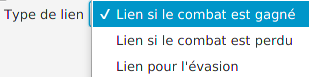
\includegraphics[width=4cm]{img/lienCombat.png}
		\end{minipage}

	\subsection{Lien noeud aléatoire}\label{subsection:lienAléatoire}
		Si le premier noeud cliqué est un noeud aléaoire, un champ de texte permet de renseigner le nombre chance pour aller vers ce lien. L'utilisateur pourra alors laisser libre court à son imagination afin de créer des chemins aléatoire.\\

		\begin{figure}[H]
			\centering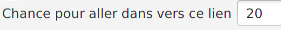
\includegraphics[width=4cm]{img/lienAleatoire.png}
		\end{figure}


	\subsection{Modification des liens}
		Une modification des liens se fait grâce au mode 
\includegraphics[height=10pt]{img/modeSelected.png}. Un simple double clique sur le lien est necessaire pour modifier ce dernier.

	\subsection{Suppression des liens}
		Ces liens, sauf le lien du prélude, peuveut être supprimés à l'aide du mode 
\includegraphics[height=0.4cm]{img/modeSupression.png}. Un simple clique sur le lien est alors necessaire. Une boite de dialog va alors s'ouvrir permettant de vérifier si l'utilisateur est bien sûr de son action.
		Si c'était un lien de combat, le type de ce lien est alors libre.
